% !TEX TS-program = pdflatex
% !TEX encoding = UTF-8 Unicode

% This is a simple template for a LaTeX document using the "article" class.
% See "book", "report", "letter" for other types of document.

\documentclass[12pt]{article} % use larger type; default would be 10pt
\usepackage{color}
\usepackage[utf8]{inputenc} % set input encoding (not needed with XeLaTeX)

%%% Examples of Article customizations
% These packages are optional, depending whether you want the features they provide.
% See the LaTeX Companion or other references for full information.

%%% PAGE DIMENSIONS

%\usepackage[top=20mm,right=20mm,bottom=15mm,left=20mm]{geometry}
% \geometry{margins=2in} % for example, change the margins to 2 inches all round
% \geometry{landscape} % set up the page for landscape
%   read geometry.pdf for detailed page layout information

\usepackage{graphicx} % support the \includegraphics command and options

% \usepackage[parfill]{parskip} % Activate to begin paragraphs with an empty line rather than an indent

%%% PACKAGES
\usepackage{booktabs} % for much better looking tables
\usepackage{array} % for better arrays (eg matrices) in maths
%\usepackage{paralist} % very flexible & customisable lists (eg. enumerate/itemize, etc.)

%\usepackage{subfig} % make it possible to include more than one captioned figure/table in a single float
\usepackage{amsfonts}
\usepackage{amsthm}
\usepackage{tikz}
\usepackage{amsmath}
\usepackage{float}
\usepackage{graphicx}
\usepackage{caption}
\usepackage{subcaption}
\usepackage{color}
\usepackage{amssymb}
\usepackage{bm}

% These packages are all incorporated in the memoir class to one degree or another...

%%% HEADERS & FOOTERS
\usepackage{fancyhdr} % This should be set AFTER setting up the page geometry
\pagestyle{fancy} % options: empty , plain , fancy
\renewcommand{\headrulewidth}{0pt} % customise the layout...
\lhead{}\chead{}\rhead{}
\lfoot{}\cfoot{\thepage}\rfoot{}

%%% SECTION TITLE APPEARANCE
%\usepackage{sectsty}
%\allsectionsfont{\sffamily\mdseries\upshape} % (See the fntguide.pdf for font help)
% (This matches ConTeXt defaults)

%%% ToC (table of contents) APPEARANCE
%\usepackage[nottoc,notlof,notlot]{tocbibind} % Put the bibliography in the ToC
%\usepackage[titles,subfigure]{tocloft} % Alter the style of the Table of Contents
%\renewcommand{\cftsecfont}{\rmfamily\mdseries\upshape}
%\renewcommand{\cftsecpagefont}{\rmfamily\mdseries\upshape} % No bold!


\newtheorem{theorem}{Theorem} 
\newtheorem{lemma}{Lemma}
\newtheorem{propn}{Proposition}
\newtheorem*{thmm}{Theorem}
\newtheorem{remk}{Remark} 
\newtheorem{corol}{Corollary}
\newtheorem{definition}{Definition}



\newtheorem{thm}{Theorem}[section] 
\newtheorem{prop}[thm]{Proposition} 
\newtheorem{lem}[thm]{Lemma}
\newtheorem{cor}[thm]{Corollary} 
\newtheorem{con}[thm]{Conjecture} 

\theoremstyle{definition}
\newtheorem{defn}[thm]{Definition}
\newtheorem*{rem}{Remark}
%\newtheorem*{nota}{Notation}
\newtheorem*{nota}{Notation}
\newtheorem{cla}[thm]{Claim}
\newtheorem{ex}[thm]{Example}
\newtheorem{exs}[thm]{Examples}
\newtheorem*{exer}{Exercise}
\newtheorem{case}{Case}
\newtheorem{conj}{Conjecture}

\definecolor{sotonblue}{rgb}{0.0,0.394,0.597}


%opening
 \title{Nine Month Report}
\author{David Matthews \\\\\emph{Supervisors: Dr James Anderson and Dr Ben MacArthur}}

\begin{document}
 
\maketitle
 
Graph Theory has been an established area of discrete mathematics since 1736 when Euler solved the famous question regarding the bridges of K\"{o}nigsberg.  More recently, in the 1940s and 50s Erd\H{o}s and R\'{e}nyi laid the foundations of the theory of random graphs seeking to answer fundamental questions about the nature of ``most'' graphs. Random graphs have been studied for their own sake and have been used to model a diverse set of real-world networks from the world wide web to the metabolism of \emph{E. coli}. Recently, the advent of the world wide web and the accompanying %symbiotic?
(relatively) cheap and powerful computational power has led to a reemergence of graph and random graph theory under the guise of ``Network Science''. 
  
During the last nine months I have divided my attention between two projects which both pertain to random trees.  The first project is entitled \emph{the expected automorphism group of random recursive trees} and is an investigation into the relationship between a variation of the usual Fibonacci sequence and a family of randomly generated trees. We will refer to this project as \emph{Project 1}. The second project is a continuation of my MSc dissertation which focused on a graph theoretical model of the cerebral vasculature.  We will refer to this project as \emph{Project 2}. Project 2 came about because of an interdisciplinary collaboration between Dr James Anderson in mathematics, Dr Roxana Carare who is an Alzheimer's disease specialist from the Faculty of Medicine and myself.  This collaboration was facilitated by the Web Science doctoral training centre. 

%\section{Notation}%these need to go in the appropriate places for now.  Later they will be changed.
%\begin{itemize}
% \item[$\bm{1}$] - The column vector such that every component is a 1.  
% \item[$S_{j}$] - The symmetric group on $j$ elements.
% \item[$k_{jk}$] - A bipartite graph
% \item[$(A^{n})_{ij} $] - The element in the $i^{th}$ row and the $j^{th}$ column of the matrix $A^{n}$.
% \item[I] - The identity matrix.
% \item[$v,v^{T}$] - A vector $v$ is always defined to be a column vector and $v^{T}$ is the transpose of $v$ (a row vector).
%\end{itemize}


\section{Introduction to Project 1}\label{aut}

Given a family of algebraic structures, $A$, it is important to know when $a_{1},a_{2} \in A$ can be considered ``the same'' and to make precise the notion of breaking $A$ into simpler pieces. Therefore we make three vital definitions in this section: random recursive trees (RRTs), RRT isomorphisms and induced subtrees. 

A graph $G$ is an ordered pair of disjoint sets $(V,E)$ such that $E$ is a subset of unordered pairs of elements of $V$. We say that $V(G)$ is the set of vertices or nodes of $G$ and that $E(G)$ is the set of edges of $G$ \cite{Bela}.
 
A \emph{random recursive tree} (RRT), $T$, with vertices $V(T) = \{v_{1},\dots,v_{n}\}$ is a labelled, rooted tree obtained by assigning a root vertex $v_{1}$ then adding $n-1$ vertices one by one such that each new vertex is joined by an edge to a randomly and uniformly chosen existing vertex. A random recursive $q$-ary tree is a labelled, rooted tree built in the same way as a random recursive tree except each new vertex is attached uniformly at random to an existing vertex that has outdegree less than $q$ \cite{Berg}.  We say that RRTs and random recursive $q$-ary trees are \emph{increasing} trees.  

It is natural to consider increasing trees as increasing tree \emph{processes} which are nested sequences of rooted, labelled trees
\[T_{1} \subset T_{2} \subset \dots \subset T_{n}\]
Where each $T_{t}$ has precisely $t$ nodes (and $(t-1)$ edges).  At time $t$ vertex $v$ is chosen from $V(T_{t-1})$  according to the appropriate attachment model and a new vertex $v_{t}$ is attached to $T_{t-1}$ via the edge $\{(v,v_{t})\}$.

\begin{ex}
For a RRT the appropriate attachment model is uniformly random random attachment.  Since there are $(n-1)!$ possible sequences $(T_{t})_{1}^{n}$, the RRT processes space can be made into a probability space by choosing each possible sequence equiprobably. 
\end{ex}
 
Let $T_{n}$ be a random recursive tree with root $v_{1}$.  For any $ v \in V(T_{n})$ such that $ v \neq v_{1}$ let the set of vertices $U_{v}$ be such that the shortest path from $u \in U_{v}$ to $v$ does not contain $v_{1}$. We say that $B(v) = U_{v} \cap v_{1}$ is the \emph{branch} containing $v$. We define $B(v_{1}) =  V(T_{n})$.     

Given an increasing tree $T_{n}$ on $n$ vertices labelled by the function $\phi : V(T) \rightarrow \{1,2,\dots,n\}$ and a vertex $v \in V(T)$ then we can consider $\tilde{T_{v}}$  which is the induced subtree with vertices, $v_{i}\in B(v)$ such that $\phi(v_{i}) \geq \phi(v)$. 

 \begin{figure}[h]
\centering
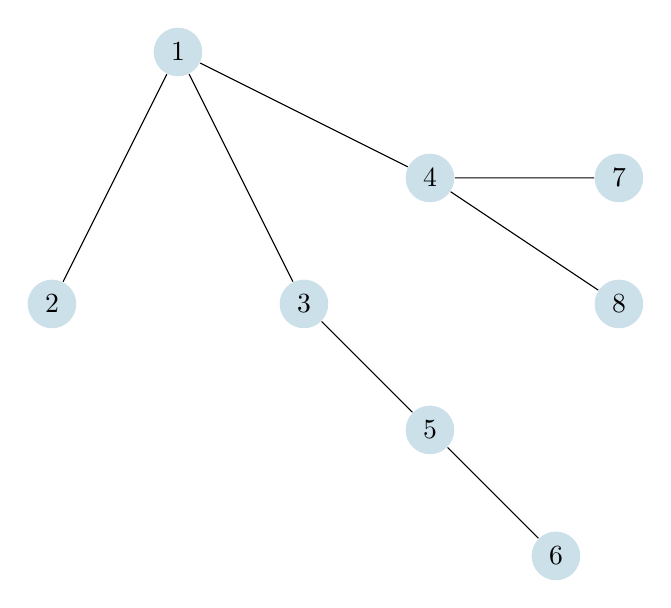
\begin{tikzpicture}
  [scale=0.8,auto=left,every node/.style={circle,fill=sotonblue!20}]
  \node (n1) at (3,10) {1};
  \node (n2) at (1,6)  {2};
  \node (n3) at (5,6)  {3};
  \node (n4) at (7,8) {4};
  \node (n5) at (7,4)  {5};
  \node (n6) at (9,2)  {6};
  \node (n7) at (10,8)  {7};
  \node (n8) at (10,6)  {8};

  \foreach \from/\to in {n1/n2,n1/n3,n1/n4,n5/n3,n5/n6,n4/n7,n4/n8}
    \draw (\from) -- (\to);

\end{tikzpicture}
\caption{An example of a random recursive tree on 8 vertices.  The induced subtree $T_{v_{4}}$  consists of vertices $v_{4},v_{5},v_{6}$ and edges $\{(v_{4},v_{7}),(v_{4},v_{8})\}$. }
\end{figure}
 
An automorphism of a graph is a permutation of the vertices of that graph which preserves adjacency (two vertices are said to be adjacent if there exists an edge joining them). 

Numerical analysis conducted by  MacArthur of 50 independent sequences in which the median value of $Aut(T_{n})$ was calculated yielded the following conjecture.\footnote{We have confirmed MacArthur's numerical analysis using the graph isomorphism software \emph{nauty}.}%we have extended this result and done it for preferential attachment models as well.

\begin{conj}\label{conj1}
Let $(T_{t})_{0}^{n}$  be a RRT process, then almost surely 
\[\lim_{n \rightarrow\infty} |Aut(T_{n})|^{\frac{1}{n}} \rightarrow \nu\]
where $\nu \sim 1.13198824$ is Viswanath's constant \cite{Bens}.
\end{conj}

Viswanath's constant arises from the following simple adaptation of the Fibonacci sequence.  Let $f_{1} = f_{2} = 1$ as usual and for $t>2$ let $f_{t} = f_{t-2} \pm f_{t-1}$ where the plus and minus are chosen with probability $1/2$.  Viswanath showed that almost surely $|f(t)|^{\frac{1}{t}} \rightarrow 1.13198824 $ as $t\rightarrow\infty$ although his proof was computational in nature \cite{Viswanath}.  We aim to prove Conjecture \ref{conj1} and to derive Viswanath's constant analytically. 



\subsection{The automorphism group of random recursive trees}

It is a result of P\'{o}lya that the automorphism group of a tree belongs to the class of permutation groups which contains the symmetric groups and is closed under taking direct and wreath products \cite{biggs:1993}. So there exists a direct product decomposition for any increasing tree $T_{n}$:
 \begin{equation}\label{decomp}
  Aut(T_{n}) = A_{1} \times A_{2} \times\dots\times A_{p} \times B_{1} \times B_{2} \times \dots \times B_{q}
 \end{equation}
Such that $A_{i} \cong S_{x(i)}$ and $B_{j} = S_{y_{1}(j)} \wr S_{y_{2}(j)} \wr \dots \wr S_{y_{k_{j}}(j)}$.

In addition to this algebraic interpretation of $Aut(T_{n})$ there is a pleasing geometric realisation of equation \ref{decomp} in which each symmetric factor $A_{i}$ corresponds to a hub vertex adjacent to $k$ paths of length $n$, each of which terminates in a leaf vertex which we say is a $(n,k)$-star.  On the other hand each $B_{i}$ corresponds to an extended symmetric induced subtree \cite{Ben}. 

\begin{ex}

\begin{figure}[H]
\centering
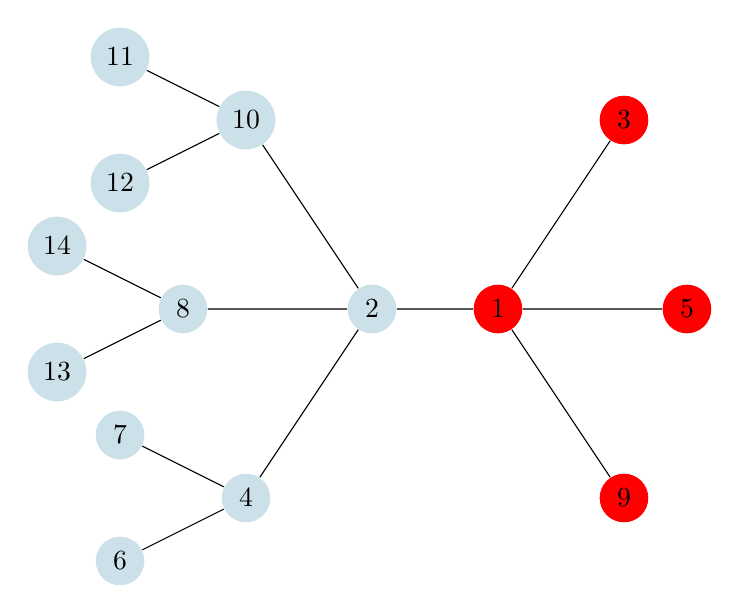
\begin{tikzpicture}
  [scale=0.8,auto=left,every node/.style={circle,fill=sotonblue!20}]

  \node[style={circle,fill=red!100}] (n1) at (7,5) {1};
  \node (n2) at (5,5)  {2};
  \node[style={circle,fill=red!100}] (n3) at (9,8)  {3};
  \node (n4) at (3,2) {4};
  \node[style={circle,fill=red!100}] (n5) at (10,5)  {5};
  \node (n6) at (1,1)  {6};
  \node (n7) at (1,3)  {7};
  \node (n8) at (2,5)  {8};
  \node[style={circle,fill=red!100}] (n9) at (9,2)  {9};considering
  \node (n10) at (3,8)  {10};
  \node (n11) at (1,9)  {11};
  \node (n12) at (1,7)  {12};
  \node (n13) at (0,4)  {13};
  \node (n14) at (0,6)  {14};
  \foreach \from/\to in {n1/n2,n1/n3,n1/n5,n1/n9,n2/n4,n2/n8,n2/n10,n10/n11,n10/n12,n8/n14,n8/n13,n4/n7,n4/n6}
    \draw (\from) -- (\to);
\end{tikzpicture}
\caption{An example of a random recursive tree, $T_{14}$ such that $Aut(T) \cong S_{3} \times S_{2}\wr S_{3}$.  The red vertices indicate an induced subtree $\tilde{T}_{v_{1}}$ isomorphic to the bipartite graph $k_{1,3}$ which contributes $S_{3}$ to $Aut(T_{14})$. The blue nodes highlight an induced subtree, $\tilde{T}_{v_{2}}$ of $T_{14}$ isomorphic to an extended symmetric subtree and contributes $S_{2}\wr S_{3}$ to $Aut(T)$.}\label{fig2}
\end{figure}

\end{ex}
%In section \ref{onestars} we calculate the expected size of, $Aut_{1}(T_{n}^{q})$,  the subgroup of $Aut(T_{n}^{q})$ contributed to by 1-stars.  Note that every $k$-star is an induced subtree $T'$ of $T$ such that $T'\cong k_{1,k}$ a bipartite graph with a hub and $k$ leaves.   
 

 
Let $(T_{t})_{1}^{n}$ be a RRT process with root $v_{1}$ and labbeling $\phi$.  Consider any induced subtree $\tilde{T}_{v} \cong k_{1,p}$ of $T_{n}$ with the vertex set $V(\tilde{T}_{v}) = \{v,v_{1}',v_{2}',\dots,v_{p}'\}$.  By the definition of an induced subgraph $v_{1}',v_{2}',\dots,v_{p}'$ are leaves of $T_{n}$.  If either $v_{1} \notin V(\tilde{T}_{v})$ or $v = v_{1}$ then $\phi (v) < \phi (v_{j}')$ for all $j$.  However, if $v_{1} \in V(\tilde{T}_{v}) \diagdown \{v\}$ then $\phi(v) \nless \phi(v_{j}')$ for all $j$.

For $t>1$ the probability that $v_{1}$ is a leaf is $\frac{1}{t-1}$.  So as $n \rightarrow\infty$:
\[\mathbb{P} (\text{ that there exists a  }  \tilde{T}_{v} \text{  such that  }  \phi(v) \nless \phi(v_{j}') \text{  for all  } j \rightarrow 0)\rightarrow 1\]
 
\subsection{Generalised P\'{o}lya Urns}\label{Gen}
The decomposition of automorphism group described by Equation \ref{decomp} provides a way of proving Conjecture \ref{conj1}. It is enough to enumerate the expected proportion of $(n,k)$-stars and extended symmetric branches of an RRT to calculate the expected automorphism group.  Since P\'{o}lya urn processes (defined below) have been used to calculate various features of RRTs such as degree distribution and expected depth of vertices they are a viable method for this enumeration.  
 
 A generalised P\'{o}lya urn process, $(X_{t})_{t=0}^{\infty}$, is defined to have $q$ types $1,2,\dots,q$ and $X_{t} = (X_{t1},\dots,X_{tq})$ such that $X_{ti}$ is the number of balls of type $i$ in the urn at time $t$.  Initially the urn's contents are described by $X_{0}$ (deterministic or random).  For each type $i$ we associate an activity $a_{i}$ and an expectation transition vector $\mathbb{E}(\xi_{i}) = (\xi_{i1},\dots,\xi_{iq})$.  At each time $t\geq 1$ one of the balls is chosen at random from the urn and the probability of drawing a ball of type $i$ at time $t$ is 
 \[                                                                                                                                                                                                                                                                                                                                                                                                                                                                                                                                                                                   \frac{a_{i}X_{(t-1),i}}{\sum_{j}a_{j}X_{(t-1),j}}.
 \]                                                                                                                                                                                                                                                                                                                                                                                                                                                                                                                                                                                                                                                                                                                                                                                                                                                                                                                                                                                                                                                             
Note that if every $a_{i} = 1$ then the balls are chosen uniformly at random.  Once a ball of type $i$ has been chosen it is                                                                                                                                                                                                                                                                                                                                                                                                                                                                                                                                                                                                                                                                                                                                             returned to the urn with $Y_{tj}$ balls of type $j$ where $\mathbb{E}(Y_{tj})= \xi_{ij}$ \cite{JansonSPATA}.
 
Let $A$ denote the $q \times q$ matrix
\[A = \left(a_{j}\mathbb{E}(\xi_{ji})\right)^{q}_{i,j = 1}.\]

Let $\Lambda$ be the set of eigenvalues of $A$. The eigenspectrum of $A$ will play a central role in the limiting behaviour of the urn process.  
\subsection{Properties of $A$}
 
 We write $i\succ j$ if $(A^{n})_{ji} > 0 $ for some $n \geq 0$.  Note that $\succ$ is transitive and reflexive so it partitions the set of types into equivalence classes $C_{p}$ such that $i,j$ are in the same equivalence class if $i\prec j \succ i$.  We say that type $i$ is \emph{dominating} if $i \succ j$ for every type $j$.  Similarly a class $C_{k}$ is said to be \emph{dominating} if every $i \in C_{k}$ is dominating.   

The usual assumptions one makes for an urn process are:
\begin{itemize}
 \item[(A1)] $\xi_{ij} + \delta_{ij} \geq 0$ a.s. for all $i,j$.
 \item[(A2)] $\mathbb{E}(\xi_{ij}) < \infty$ for all $i,j$.
 \item[(A3)] There exists a largest real eigenvector $\lambda_{1}$ such that $\lambda_{1} >0$.
 \item[(A4)] $\lambda_{1}$ is simple.
 \item[(A5)] There exists a dominating type, $i$ and $X_{0i} >0$.
 \item[(A6)] $\lambda_{1}$ belongs to the dominating class.
 \end{itemize}

 An urn process which satisfies (A1)-(A6) is called irreducible and tenable.  We say that the left and right eigenvectors corresponding to $\lambda_{1}$ are $u_{1}$ and $v_{1}$ respectively.
 
\subsection{Limiting Behaviour} 
 
A generalised P\'{o}lya urn scheme can be embedded in a multi-type continuous time Markov branching process $\chi(t) = (\chi_{1}(t), \dots, \chi_{q}(t))$ with initial vector $\chi(0) = X_{0}$.  In this process particles of type $i$ live for an expected time of $a_{i}^{-1}$ (with exponential distribution).  When a particle of type $i$ dies it is replaced with a set of particles with distribution given by $(\xi_{ij} + \delta_{ij})_{j=1}^{q}$ \cite{Athreya}.  

Let $\tau_{0} = 0$ and $\tau_{n}$, $n \geq 1$ be the $n^{th}$ time %not sure about this
a ball dies. The P\'{o}lya urn process $(X_{n})_{n=0}^{\infty}$ equals in distribution the process $(\chi(\tau_{n}))_{n=0}^{\infty}$ so limit theorems for $X_{n}$ can be derived from limit theorems for $\chi(t)$ - see Chapter V of \cite{Athreya}.
 
Assume that $A$ is tenable and irreducible.  By Theorem 7.6 in \cite{linalg}, there exists a direct sum decomposition of $\mathbb{C}^{q}$ as $\bigoplus E_{\lambda}$ of eigenspaces $E_{\lambda}$ and there exist projections $P_{\lambda}$ for every eigenvalue $\lambda$ of $A$ that satisfy $\sum_{\lambda \in \Lambda}P_{\lambda} = I$ and $ AP_{\lambda} = \lambda P_{\lambda} + N_{\lambda}$.  Where $N_{\lambda}$ is nilpotent. Let $d_{\lambda} \geq 0 $ be the least integer such that $N_{\lambda}^{d_{\lambda}} \neq 0$.  For $k = 0,1,2,\dots$ we define the quotient space $E_{\lambda,k}: = E_{\lambda}/N_{\lambda}^{k+1}E_{\lambda}$ and the projection $Q_{\lambda,k}:E_{\lambda} \rightarrow E_{\lambda,k}$.
 
In particular $P_{\lambda_{1}}$ and $Q_{\lambda_{1},0}$ are \cite{JansonSPATA}:
\begin{equation}\label{eq5}
 P_{\lambda_{1}} = v_{1}u_{1}^{T},\text{           } Q_{\lambda_{1},0} = I
\end{equation}
 
In \cite{JansonSPATA}, Lemma 9.2, Janson defines the following martingale if $t \geq 0$.
 
\[
 \mathcal{Y}(t) = e^{-tA}\chi(t) = \sum_{j=0}^{\infty} \frac{t^{j}A^{j}}{j!}\chi(t)
\]

\begin{lem}\label{lemlam}
 If $Re{\lambda} > \lambda_{1}/2$ for any $\lambda \in \Lambda$ then there exists a random vector $\tilde{W}_{\lambda} \in E_{\lambda}$ such that $P_{\lambda}\mathcal{Y}(t) \rightarrow \tilde{W}_{\lambda}$ almost surely as $t \rightarrow\infty$ %in $L^{2}$. 
\end{lem}
\begin{proof}
 See Lemma 9.5 in \cite{JansonSPATA}
\end{proof}
We also make the following definitions:
\begin{equation}
 W_{\lambda} = Q_{\lambda,0}\tilde{W}_{\lambda}.
\end{equation}
\begin{equation}
 W = u_{1} \cdot W_{\lambda_{1}}
\end{equation}
%What should be t or n?

 \begin{thm}\label{th1}\cite{Janson}
 If a generalised P\'{o}lya urn is irreducible and tenable and $\sum a_{j}\xi_{j} = m$ for $j = 0,1,\dots,q$ and $m >0$ then almost surely
 \[t^{-1}X_{t} \rightarrow \lambda_{1}v_{1} \text{    as   } t \rightarrow\infty\]
 Since the choice of $v_{1}$ is unique up to scalar factor we normalise such that $a \cdot v_{1} = 1$. 
\end{thm}

In section \ref{onestars} we will relax condition (A1) and just require that the urn process never allows balls to be removed from the urn unless those balls exist. %write this mathematically.  
In  order that Theorem \ref{th1} holds we must show (\cite{JansonSPATA}, Remark 4.2):
\begin{itemize}
 \item[ (B1)] There exists left and right eigenvectors $u_{1}$ and $v_{1}$ of $\lambda_{1}$ such that for every $i$ in the dominating class $v_{1i} > 0$ and $u_{1i}>0$.
 \item[(B2)] $\mathbb{P}(u_{1}.\mathcal{Y}(t) > 0 \text{  and  } W = 0) \rightarrow 0$ almost surely as $t \rightarrow \infty.$
 \item[(B3)] (A2)-(A6) hold.
\end{itemize}

\section{$(1,k)$-stars}\label{onestars}
 
 
 
 In this section we will describe a P\'{o}lya urn which will calculate the number of 1-stars of a random recursive $q$-ary tree, $T_{n}^{q}$ for some fixed $q >3$, rooted at $v_{0}$ with labelling  $\phi$.  Balls in this urn scheme take exactly one of $q+1$ types and each ball corresponds to a node in a random recursive $q$-ary tree. Balls of types $j = 1,2,3,\dots,q$ correspond to a vertex of an induced subtree $\tilde{T}_{v}\cong k_{1,j}$ with vertex set $V(\tilde{T}_{v}) = \{ v,v_{1}',v_{2}',\dots,v_{j}'\}$ such that $\phi(v) < \phi(v_{p}') $ for $p = 1,2,\dots,q$. Balls of type 0 correspond to any other node in $V(T_{n})$. 
 
 \begin{ex}
  The P\'{o}lya urn corresponding to $T_{14}$ depicted in Figure \ref{fig2} would contain 1 ball of type 0, 9 balls of type 2 and 4 balls of type 3. 
  
  \begin{figure}[H]\label{fig3}
\centering
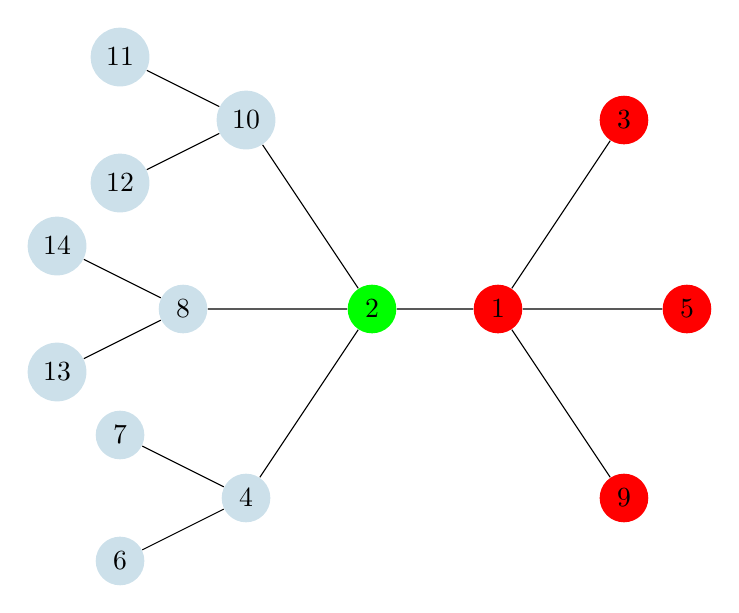
\begin{tikzpicture}
  [scale=0.8,auto=left,every node/.style={circle,fill=sotonblue!20}]

  \node[style={circle,fill=red!100}] (n1) at (7,5) {1};
  \node[style={circle,fill=green!100}] (n2) at (5,5)  {2};
  \node[style={circle,fill=red!100}] (n3) at (9,8)  {3};
  \node (n4) at (3,2) {4};
  \node[style={circle,fill=red!100}] (n5) at (10,5)  {5};
  \node (n6) at (1,1)  {6};
  \node (n7) at (1,3)  {7};
  \node (n8) at (2,5)  {8};
  \node[style={circle,fill=red!100}] (n9) at (9,2)  {9};considering
  \node (n10) at (3,8)  {10};
  \node (n11) at (1,9)  {11};
  \node (n12) at (1,7)  {12};
  \node (n13) at (0,4)  {13};
  \node (n14) at (0,6)  {14};
  \foreach \from/\to in {n1/n2,n1/n3,n1/n5,n1/n9,n2/n4,n2/n8,n2/n10,n10/n11,n10/n12,n8/n14,n8/n13,n4/n7,n4/n6}
    \draw (\from) -- (\to);
\end{tikzpicture}
\caption{The 4 red vertices indicate an induced subtree $\tilde{T}_{v_{1}}$ isomorphic to the bipartite graph $k_{1,3}$ which contributes 4 balls of type 3 to the urn.  The blue nodes indicate 3 induced subtrees of $T_{14}$ isomorphic to $k_{1,3}$ and contribute 9 balls of type 2 to the urn.  The green node corresponds to 1 ball of type 0 in the generalised P\'{o}lya urn.}\label{fig3}
\end{figure}
 \end{ex}

 %draw some example trees and explain (O.M.Tree)
 
At time $t$ for $t = 0,1,2,3,\dots$ the contents of the urn are described by the $q+1$ dimensional vector $X_{t} = (X_{t0},X_{t1}, \dots X_{tq})$ such that each $X_{tj}$ is defined to be the number of balls of type $j$ in the urn at time $t$.  Initially we set $X_{0} = (1,0,0,\dots,0)$ which corresponds to the tree with one vertex and no edges. 

We also assign an activity $a_{j} = 1$ to every type $j$ (recall that this means that balls are picked from the urn uniformly at random) and an expectation transition vector $\mathbb{E}(\xi_{j})$  to every type in the way we described in section \ref{Gen}.  Each expectation transition vector is of the form  $\mathbb{E}(\xi_{j}) = (\xi_{j0},\xi_{j1},\dots,\xi_{jq})$,  where $\xi_{jk} + \delta_{jk}$ corresponds to the expected number of nodes of type $k$ created when a vertex of type $j$ is chosen for attachment.
 
 
Note that the expectation transition vector has a general form for $j = 3,4,\dots,q-1$ and is more complicated otherwise. We will deal with the atypical cases first.  

If a ball of type 1 is drawn from the urn at time $t$ this corresponds to node $v_{t}$ being attached to some induced subtree $\tilde{T}' \cong k_{1,1}$.  Let $V(\tilde{T}') = \{v_{1},v_{2}\}$ such that $\phi(v_{1}) < \phi(v_{2})$, the probability of attaching $v_{t}$ to $v_{1}$ is 0.5 and the probability of attaching to $v_{2}$ is 0.5.  If $v_{t}$ is attached to $v_{1}$ then the three vertices $\{v_{1},v_{2},v\}$ become part of a new subtree $\tilde{T}^{(2)} \cong k_{1,2}$ .  If $v_{t}$ is attached to $v_{2}$ then $v_{1}$ corresponds to ball of type 0 and $v_{1}$ and $v$ are the vertices of a new induced subtree $\tilde{T}^{(3)}\cong k_{1,1}$.  This can be expressed in terms of $\xi_{ij}$ as follows.
 \[
   \mathbb{E}(\xi_{1}) = 1/2(1,0,\dots,0) + 1/2(0,-2,3,0 \dots, 0) 
 \]
 
 %add another diagram here you monster
 
In a similar way we found that:
 \begin{align}
  \mathbb{E}(\xi_{0}) &= (-1,2,0,\dots,0)\\
   \mathbb{E}(\xi_{1}) &= (\frac{1}{2}, -1, \frac{3}{2},0,\dots,0)\\
  \mathbb{E}(\xi_{2}) &= (0,\frac{8}{3}, -3,\frac{4}{3},0,\dots,0)\\
  \mathbb{E}(\xi_{q}) &= (0,\frac{2q}{(q+1)},0,\dots,0,\frac{q^{2}}{(q+1)}, -q)\\
 \end{align}
 
On the other hand, if one was to pick a ball of type $j = 3,4,\dots q-1$ from the urn at time $t$ this corresponds to a probability of $\frac{1}{j+1}$ that one attaches $v_{t}$ to the hub of the corresponding induced subgraph $ T' \cong k_{1,j}$ and a probability of $\frac{j}{j+1}$ that one attaches $v_{t}$ to a leaf of $T$.  Therefore, the appropriate transition vectors are of the form:
\begin{align}
 \xi_{j1} &= \frac{2j}{j+1}\\
 \xi_{j(j-1)} &= \frac{j^{2}}{(j+1)},\\ 
 \xi_{jj} &= -(j+1)\\
 \xi_{j(j+1)} &= \frac{(j+2)}{(j+1)}\\
 \xi_{jk} &= 0 \text{   otherwise} \\
\end{align}

We can then make matrix $A_{q}$ as described in section \ref{Gen}. 

\begin{ex}
 \begin{equation}
  A_{5} = \left(
  \begin{matrix}
  -1 & \frac{1}{2} & 0 & 0 & 0 & 0 \\
  2 & -1 & \frac{8}{3} & \frac{6}{4} & \frac{8}{5} & \frac{10}{6} \\
  0 & \frac{3}{2} & -3 &\frac{9}{4} & 0 & 0 \\
  0 & 0 & \frac{4}{3} & -4 & \frac{16}{5} & 0 \\
  0 & 0 & 0 & \frac{5}{4} & -5 & \frac{25}{6} \\
  0 & 0 & 0 & 0 & \frac{6}{5} & -5 
  
 \end{matrix}
 \right)
\end{equation}
\end{ex}




\subsection{Bounds for $v_{1}$}\label{sec:bounds}
To find $v_{1}$ we must solve $A_{q}v_{1} = \bm{1}v_{1}$, which we can consider as a set of $q+1$ simultaneous equations which we will label $(E_{0}) - (E_{q})$.   
We find bounds for the $v_{j}$ using a series of inequalities.

Note that by $E_{0}$ and $E_{q}$:
\begin{equation}\label{eq3}
 v_{1} = 4v_{0} \text{    and    } v_{q-1} = qv_{q}.
\end{equation}

\begin{lem}\label{lem:bounds1}
 For $j = 1,2,\dots,q-2$ 
 \[v_{j} > \frac{q!v_{q}}{j!}\]
\end{lem}
\begin{proof}
By $E_{q-1}$: 
\[
 \frac{q}{q-1} v_{q-2} + \frac{q^{2}}{q+1}v_{q} = (q+1)v_{q-1} 
\]

By re-aranging and using equation \ref{eq3} we found that,
\begin{equation}\label{eq1}
\frac{v_{q-2}}{q-1}  = (1 + \frac{1}{q} - \frac{1}{q+1})v_{q-1} > v_{q-1}.
\end{equation}

We assume for the inductive hypothesis that for $n=1,2,3,4,\dots,k-1$:
\[\frac{v_{q-n-2}}{q-n-1} > v_{q-n-1}\]
We have already proved the base case (equation \ref{eq1}) when $n=0$.

Consider $E_{q - k - 1}$:
\[\frac{q - k}{q-k -1} v_{q-k-2} + \frac{(q-k)^{2}}{q-k+1}v_{q-k} = (q-k+1)v_{q-k-1}  \] 

By the inductive hypothesis we have that:
\[\frac{v_{q-k-2}}{q-k-1} > (1 + \frac{1}{q-k} - \frac{1}{q-k+1})v_{q-k-1} > v_{q-k-1}\]

So for $j = 1,2,3,\dots, q-2$ 
\begin{equation}\label{eq2}
v_{j} > (j+1)v_{j+1} > \dots > (j+1)(j+2)\dots (q-1)v_{q-1} = \frac{q!}{j!}v_{q}
\end{equation}
\end{proof}

\begin{lem}\label{lem:bounds2}
  For $j = 1,2,3,\dots,q-2$ 
  \[v_{j} < \frac{qq!(j+1)}{(j+1)!(q+1)}v_{q}\]
 \end{lem}
\begin{proof}
We will prove this lemma in a similar manner to lemma \ref{lem:bounds1}.  For the base case we can rearange $E_{q-1}$ and use equation \ref{eq3} to find that $v_{q-2} < \frac{q^{2}}{q+1}v_{q-1}$.
 
For the inductive hypothesis assume that $ v_{q-n-1} < \frac{(q-n+1)^{2}}{q-n+2}v_{q-n}$ for $n = 1,2,3,\dots k$.  Using the inductive hypothesis we can rearrange $E_{q-k-1}$:
\begin{align}\label{eq:1}
  v_{q-k-2} &= \frac{q-k-1}{q-k}\left((q-k+1)v_{q-k-1} - \frac{(q-k)^{2}}{(q-k+1)}v_{q-k} \right) \\
  &< \frac{q-k-1}{q-k}\left((q-k+1)- \frac{(q-k)^{2}(q-k+2)}{(q-k+1)^{3}} \right)v_{q-k-1} \\
  &= \left(q- k + 1 -1 -\frac{1}{(q-k)} - \frac{(q-k)^{2}(q-k+2)}{(q-k+1)^{3}} \right)v_{q-k-1} \\
  &= \left( \frac{(q-k+1)((q-k)^{2}-1)}{(q-k)(q-k+1)} - \frac{(q-k)^{2}(q-k+2)}{(q-k+1)^{3}} \right)v_{q-k-1} \\
  &= \left( \frac{(q-k)^{2}}{q-k+1} + \frac{1}{(q-k)(q-k+1)} - \frac{1}{q-k+1} - \frac{(q-k)^{2}(q-k+2)}{(q-k+1)^{3}} \right)v_{q-k-1} \\
  &< \frac{(q-k)^{2}}{q-k+1}v_{q-k-1}
\end{align}
 Therefore for any $j = 1,2,\dots,q-2$, by equation \ref{eq:1},
 \begin{align}
  v_{j} &< \frac{(j+2)^{2}}{(j+3)}v_{j+1} \\
  &< \frac{(j+2)^{2}(j+3)}{(j+4)}v_{j+2} < \dots < \frac{(j+2)^{2}(j+3)\dots(q-1)q}{(q+1)}v_{q-1} \\
  &= \frac{(j+2)^{2}(j+3)\dots(q-1)q^{2}}{(q+1)}v_{q} \\
  v_{j} &< \frac{q!q(j+2)}{(j+1)!(q+1)}v_{q}.
 \end{align}
 \end{proof}

\begin{lem}\label{lem:bounds3}
 For $q > X$ the following inequality holds:
 \[\frac{8}{23q!}< \frac{8(q+1)}{23q!q} < v_{q} < \frac{4}{7q!}\]
 \end{lem}
 
 \begin{proof}
 By the normalisation property discussed in Theorem \ref{th1} $\sum_{j=0}^{q}v_{i} = 1$.  Using Equation \ref{eq3} with Lemmas \ref{lem:bounds1} and \ref{lem:bounds2} we found that:
 \begin{align}
  1 = \sum_{j=0}^{q}v_{j} &< \sum_{j=1}^{q-2}\frac{qq!(j+2)v_{q}}{(j+1)!(q+1)} + v_{0} + v_{q-1} + v_{q} \\
  &<\left( \frac{qq!}{q+1}\sum_{j=1}^{q-2}\frac{(j+2)}{j+1)!} + \frac{3q!q}{8(q+1)} + q + 1 \right) v_{q}\\
  &<\left( \frac{qq!}{q+1}(1 + 2(e-2))+ \frac{3q!q}{8(q+1)} + q + 1 \right) v_{q}\\
  &<\frac{23q!q}{8(q+1)} \\
  1 = \sum_{j=0}^{q}v_{j} &> \sum_{j=1}^{q-2}\frac{q!v_{q}}{j!} + v_{0} + v_{q-1} + v_{q} \\
  &> q!v_{q} \sum_{j=1}^{q-2}\frac{1}{j!} + \frac{q!}{4}v_{q} + qv_{q} + 1v_{q} \\
  &> \frac{7}{4}qq!v_{q}
\end{align}
 
 
A simple rearangement completes the proof of Lemma \ref{lem:bounds3}.
\end{proof}

If we collect results from Lemmas \ref{lem:bounds1}, \ref{lem:bounds2} and \ref{lem:bounds3} we see that for $j = 1,2,\dots j-2$:
\begin{equation}\label{eq:9}
\frac{8}{23j!} < v_{j} < \frac{4q(j+1)}{7(j+1)!(q+1)} < \frac{4}{7j!}
\end{equation}

\begin{lem}\label{lem:4.2}
 (B1)-(B3) hold for $A$.
\end{lem}
\begin{proof}
Since $T = A + \alpha I$ is non-negative if $\alpha > q$, by Perron	-Frobenius theory $T$ is a nonnegative, irreducible matrix.  Therefore $A$ has a real, simple eigenvalue $\lambda_{1}$ (A4) such that for any other eigenvalue $\lambda$,  $Re(\lambda) < \lambda_{1}$ and the corresponding left and right eigenvectors are the only positive eigenvectors of $A$ \cite{Seneta} .  By inspection $u_{1} = (1,1,\dots,1)$ is a left eigenvector of $A$ corresponding to eigenvalue 1 (A3), since $u_{1i} > 0$ for all $i$, $\lambda_{1} = 1$. The bounds calculated above show that there exists a right eigenvector $v_{1}$ corrosponding to $\lambda_{1}$ such that $v_{1j}>0$ for $j = 0,1,2,\dots q$.  

By the defiition of this urn process (A2) is true. Every type is dominating so, in particular, type 0 is dominating and $X_{00} = 1 >0$ (A5).  There is one dominating class so $\lambda_{1}$ belongs to the dominating class (A6).  Therefore (B1) and (B3) are satisfied. 
 
For (B2) assume that $0 = W = u_{1}W_{\lambda_{1}} = \bm{1}W_{\lambda_{1}} = \bm{1} Q_{\lambda_{1},0}\tilde{W}_{\lambda_{1}}  \bm{1}I\tilde{W}_{\lambda_{1}}$ so $0 = \tilde{W}_{\lambda_{1}}$.

Note that $Re(\lambda_{1}) = 1 > \frac{1}{2}  = \frac{\lambda_{1}}{2}$ so, by Lemma \ref{lemlam} and equation \ref{eq5} almost surely $lim_{t\rightarrow\infty}P_{\lambda_{1}}y(t) \rightarrow 0$ we can rewrite this as almost surely
\[lim_{t\rightarrow\infty}(v_{1}u_{1}^{T})y(t) \rightarrow 0\] Therefore almost surely,
\[lim_{t\rightarrow\infty}y(t) \rightarrow 0.\]
This means that almost surely $\mathbb{P}(u_{1} \dot y(t) > 0 \text{  and  } W = 0)\rightarrow 0$ as $t\rightarrow\infty$.
\end{proof}

Also note that $\sum_{j=0}^{q}a_{j}\xi_{j} = 1$ which means that one ball is added each time (corresponding to making one attachment at each discrete time).  Therefore we can appeal to Theorem \ref{th1} to see that:
 \[t^{-1}X_{t} \rightarrow \lambda_{1}v_{1} \text{  almost surely,  as   } t \rightarrow\infty\]

\subsection{Automorphisms coming from 1-stars}

To achieve our glorious goal; the calculation of the cardinality of the expected automorphism of 'most' RRTs our method has been to enumerate the expected number of $(n,k)$-stars and extended symmetric branches.  As a preliminary stage we consider the subgroup, $Aut_{1}$ of the automorphism group of a random recursive $q-ary$ process on $n$ nodes that corrosponds to $(1,k)$-stars.  

\begin{thm}
 Most random recursive $q$-ary tree processes $T_{n}^{q}$, are such that $lim_{\min(n-1,q)\rightarrow\infty} |Aut_{1}(T_{n}^{q})|^{\frac{1}{n}} < \infty$. 
\end{thm}
  
\begin{proof}
 In section \ref{sec:bounds} we found bounds for the primary eigenvector, $v_{1} = (v_{10},\dots v_{1q})$, of the matrix associated with a P\'{o}lya urn process that corresponds with a random recursive $q$-ary tree process.  By Lemma \ref{lem:4.2} $v_{1j}$ is the expected proportion of nodes that are contained in induced subtrees $\tilde{T}_{v} \cong k_{1,j}$ of $T_{n}^{q}$ such that those vertices respect the ordering decribed at the beginning of section \ref{onestars} in the limit as $n \rightarrow\infty$ .  As $n$ grows this ordering no longer becomes a restriction in the limit as $n \rightarrow\infty$ the number of expected $(1,j)$-stars is $\frac{nv_{1j}}{(j+1)}$.  
 
 The contribution of a $(1,k)$-star to $Aut(T_{n}^{q})$ is $S_{j}$ so $Aut_{1}(T_{n}^{q})$ can be written as the direct product of symmetric groups. Further $|Aut_{1}(T_{n}^{q})|$ can be written as the product of factorials.  The extended P\'{o}lya urn process tells us that for most random recursive $q$-ary tree processes $T_{n}^{q}$,  
 \[lim_{n \rightarrow\infty} \mathbb{E}(|Aut_{1}(T_{n}^{q})|) = \prod_{j=2}^{\min(n-1, q)} j!^{\frac{nv_{j}}{(j+1)}}\]
 
 By Lemma \ref{lem:bounds3} we immediately have the following bounds:
 \begin{align}
  \left( \prod_{j=2}^{\min(n-1, q)} j!^{\frac{nv_{j}}{(j+1)}}\right)^{\frac{1}{n}} &< \left(\prod_{j=2}^{\min(n-1, q)} j!^{\frac{4n}{(7(j+1)!}}\right)^{\frac{1}{n}} \\
  \left(\prod_{j=2}^{\min(n-1, q)} j!^{\frac{nv_{j}}{(j+1)}}\right)^{\frac{1}{n}} &< \left(\prod_{j=2}^{\min(n-1, q)} j!^{\frac{8n}{23(j+1)!}}\right)^{\frac{1}{n}}
 \end{align}
 
 Consider the series $S  = \sum_{j=2}^{\infty} \ln\left(j!^{\frac{4}{7(j+1)!}}\right) = \frac{4}{7}\sum_{j=2}^{\infty} \frac{ln(j!)}{(j+1)!}$.  Since $S$ converges, by \cite{JonesandSinger} it is true that $\prod_{j=2}^{\infty} j!^{\frac{4n}{7(j+1)!}} < \infty$.  
 
\end{proof}

To perform a reality check with this result please note that:

\begin{equation}\label{eq6}
 \prod_{i=2}^{q}i!^{\frac{1}{(i+1)!}} = 2^{\frac{1}{6} + \frac{1}{24} + \dots}3^{\frac{1}{24} + \frac{1}{120} + \dots }\dots \sim 1.25.
 \end{equation}
Furthermore  $1.25^{\frac{8}{23}} = 1.0807...< \nu = 1.13198824$ where $\nu$ is Viswanath's constant.  


\section{Enumerating $(2,k)$ -stars}
In section \ref{onestars} we described a P\'{o}lya urn process in order to calculate in the limit the expected number of $(1,k)$-stars of an RRT.  In this section we will extend this result and use a P\'{o}lya urn method to calculate the expected number of $(2,k)$- stars.  

Let $T_{n}^{q}$ be a RRT for some fixed $q >3$, rooted at $v_{0}$ with labelling  $\phi$.  Balls in this urn scheme take exactly one of $\frac{1}{2}(q+1)(q+2)$ types and each ball corresponds to a node in a random recursive $q$-ary tree. 

Balls of types $j = 1,2,3,\dots,q$ correspond to a vertex of an induced subtree $\tilde{T}_{v}\cong k_{1,j}$ with vertex set $V(\tilde{T}_{v}) = \{ v,v_{1}',v_{2}',\dots,v_{j}'\}$ such that $\phi(v) < \phi(v_{p}') $ for $p = 1,2,\dots,q$. 

Balls of type $k > 1$ can be written uniquely as 
\[k= \sum_{j=1}^{x}(q+ 1 -j) + y\]
where $0 < y < q+1 -j$  correspond to vertices of induced subtrees of $T$ with a hub-node $v$ of outdegree $x+y$ such that $v$ is adjacent to $x$ paths of length two terminating in a leaf vertex and $v$ is also adjacent to $y$ leaves.  Balls of type 0 correspond to any other node in $V(T_{n})$.
% insert example%
\begin{ex}
\begin{itemize}
 \item [(i)] A ball of type $k = 3 = 0 + 3$ corresponds to an induced subtree isomorphic to $k_{1,3}$.
 \item[(ii)] A ball of type $k = q + 2 = \sum_{j=0}^{1}(q+ 1 -j) + 1$ corresponds to an induced subtree isomorphic to the graph shown in figure \ref{fig:4}.
\end{itemize}
\end{ex}

 \begin{figure}[h]
\centering
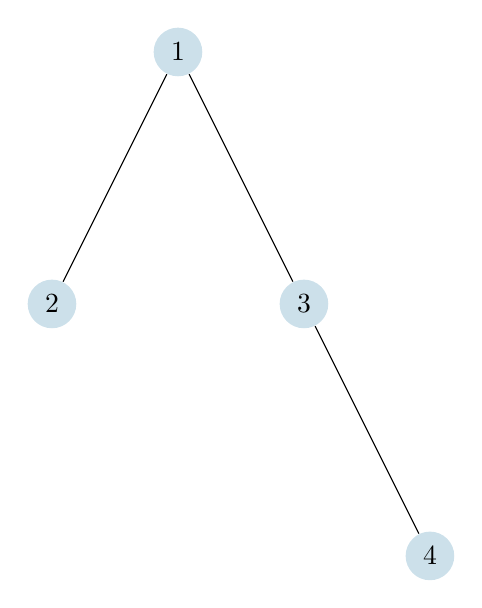
\begin{tikzpicture}
  [scale=0.8,auto=left,every node/.style={circle,fill=sotonblue!20}]
  \node (n1) at (3,10) {1};
  \node (n2) at (1,6)  {2};
  \node (n3) at (5,6)  {3};
  \node (n5) at (7,2)  {4};
\foreach \from/\to in {n1/n2,n1/n3,n5/n3}
    \draw (\from) -- (\to);
\end{tikzpicture}
\caption{}\label{fig:4}
\end{figure}

In the same way as in Section \ref{onestars} we define the expected transition probability vectors $xi_{j}$ for $j = 1,\dots,\frac{1}{2}(q+1)(q+2)$.  

The first thing to note is that $\xi_{1} = (-1,2,0,\dots,0)$ again since if we attach to a vertex that corresponds to a ball of type 0 we get two balls of type $1$.  However $\xi_{1},\xi_{2},\dots \xi_{q}$ have a different form to the transition vectors fro the P\'{o}lya urn described in section \ref{onestars}.   Assume that at time $t$  a vertex $v$ is chosen that is contained in an induced subtree isomorphic to a $(1,k)-star$  where $0<k<q$.  Then there is a probability of $\frac{1}{k+1}$ that $v$ is the hub of the $(1,k)$ - star in which case we form a $(1,k+1)$ - star i.e we add.  There is a probability of $\frac{k}{k+1}$ that $v$ is a leaf of the $(1,k)$ -star, which means that a new induced subtree with a hub adjacent to $(k-1)$ leaves and 1 path of length 2.

In terms of the transition vectors, for $0<k<q$ the following are the only non-zero components of $\xi_{k}$:
\begin{align*}
\xi_{kk} &= -(k +1) \\ 
\xi_{k(k+1)} &= \frac{k+2}{k+1} \\
\xi_{k(q+k)} &= \frac{k(k+2)}{k+1} 
\end{align*} 

%%%%Do the case 1-1-1.
If, we choose a vertex corresponding  to type $q+1$  then with probability $\frac{1}{3}$ we make a new induced subtree $\tilde{T}_{v}^{y}$ such that $v$ is adjacent to a paths of length two terminating in a leaf vertex and a leaf.  With probability $\frac{1}{3}$ we make a new induced subtree isomorphic to a $(k,2)$-star and we make one vertex with corresponding type 0.  With probability $\frac{1}{3}$ we make a new induced subtree also corresponding to type $q+1$ and we make one vertex with type 0.  

\[\xi_{q+1} = \left(\frac{2}{3},0,1,0,\dots,0,-2,\frac{4}{3},0,\dots,0\right)\]

Assume that at time $t$ we choose a vertex contained in an induced subtree, $\tilde{T}_{v}$, such that $v$ is adjacent to $x$ paths of length two terminating in a leaf vertex and $0$ leaves such that $x<q$ and $x>1$.

\begin{itemize}
\item[(i)] With probability $\frac {1}{2x +1}$ we choose $v$ and make a new induced subtree $\tilde{T}_{v}^{v}$ such that $v$ is adjacent to $x$ paths of length two terminating in a leaf vertex and 1 leaf vertex.
\item[(ii)] With probability $\frac {x}{2x +1}$ we choose a vertex distance 1 from $v$ and make a new induced subtree $\tilde{T}_{v}^{x1}$ such that $v$ is adjacent to $x-1$ paths of length two terminating in a leaf vertex and 1 leaf vertex and an induced subtree isomorphic to a $(1,2)-star$.  
\item[(iii)] With probability $\frac {x}{2x +1}$ we choose a vertex distance 1 from $v$ and make a new induced subtree $\tilde{T}_{v}^{x2}$ such that $v$ is adjacent to $x-1$ paths of length two terminating in a leaf vertex and 1 leaf vertex and an induced subtree of type $q+1$.
\end{itemize}

If $k= \sum_{j=1}^{x}(q+ 1 -j) + y$ such that $x>1$, $y=0$  thfacebooken the only non-zero components of $\xi_{k}$ are as follows:
 \begin{align*}
\xi_{k2} &= \frac{3x}{2x+1}\\
\xi_{k(q+1)} &= \frac{3x}{2x+1}\\
\xi_{kj} &= \frac{2x(2x-1)}{(2x+1)}\\
\xi_{kk} &= -2x+1 \\
\xi_{k(k+1)} &= \frac{2x + 2}{2x + 1}
\end{align*}

Such that $j= \sum_{j=1}^{x-1}(q+ 1 - j)$.

Now assume that at time $t$ we choose a vertex contained in an induced subtree, $\tilde{T}_{v}$, such that $v$ is adjacent to $x$ paths of length two terminating in a leaf vertex and $y$ leaves such that $x+y<q$ and $x,y>0$.    

\begin{itemize}
\item[(i)] With probability $\frac{y}{2x+y+1}$ we choose a leaf vertex distance 1 from $v$ and we make a new induced subtree $\tilde{T}_{v}^{y}$ such that $v$ is adjacent to $x+1$ paths of length two terminating in a leaf vertex and $y-1$ leaves.     

\item[(ii)] With probability $\frac{x}{2x+y+1}$ we choose a non-leaf vertex distance 1 from $v$ and we make a new induced subtree $\tilde{T}_{v}^{x1}$ such that $v$ is adjacent to $x-1$ paths of length two terminating in a leaf vertex and $y$ leaves and we make an induced subtree isomorphic to a $(1,2)$-star.

\item[(iii)] With probability $\frac{x}{2x+y+1}$ we choose a vertex distance 2 from $v$ and we make a new induced subtree $\tilde{T}_{v}^{x2}$ such that $v$ is adjacent to $x-1$ paths of length two terminating in a leaf vertex and $y$ leaves and we make an induced subtree isomorphic to a path of length 2.  %define a path.

\item[(iv)] With probability $\frac{1}{2x+y+1}$ we choose $v$ and we make a new induced subtree $\tilde{T}_{v}^{v}$ such that $v$ is adjacent to $x$ paths of length two terminating in a leaf vertex and $y+1$ leaves.     
\end{itemize}


Therefore if $k= \sum_{j=1}^{x}(q+ 1 -j) + y$ such that $x,y>0$,  then the only non-zero components of $\xi_{k}$ are as follows:
\begin{align*}
\xi_{k2} &= \frac{3x}{2x + y +1}\\
\xi_{k(q+1)} &= \frac{3x}{2x + y +1}\\
\xi_{kj} &= \frac{2x(2x + y -1)}{2x + y +1}\\
\xi_{kk} &= -(2x+y+ 1)\\
\xi_{kk+1}&= \frac{2x+y+2}{2x + y +1}\\
\xi_{kl} &= \frac{y(2x +y + 2)}{2x + y + 1}
\end{align*}
Such that $j = \sum_{j=1}^{x-1}(q+ 1 -j) + y$ and $l = \sum_{j=1}^{x+1}(q+ 1 -j) + y-1.$  

For the final cases assume that at time $t$ we choose a vertex of type $k$ contained in an induced subtree, $\tilde{T}_{v}$, such that $v$ is adjacent to $x$ paths of length two terminating in a leaf vertex and $y$ leaves such that $x+y=q$.  Using a similar method to section \ref{onestars} the non-zero components of $\xi_{k}$ to be:
\begin{align*}
\xi_{k2} &= \frac{3x}{2x + y +1}\\
\xi_{k(q+1)} &= \frac{3x}{2x + y +1}\\
\xi_{kj} &= \frac{2x(2x + y -1)}{2x + y +1}\\
\xi_{kk} &= -\frac{2x + y}{(2x+y+ 1)}\\
\xi_{kl} &= \frac{y(2x +y + 2)}{2x + y + 1}
\end{align*}
Such that $j = \sum_{j=1}^{x-1}(q+ 1 -j) + y$ and $l = \sum_{j=1}^{x+1}(q+ 1 -j) + y-1.$  

For simplicity we will now refer to type $k = \sum_{j=1}^{x}(q+ 1 -j) + y$ as type $\tau_{x,y}$.

Following the method of section \ref{onestars} this new P\'{o}lya urn is tenable and irreducible with principle eigenvalue $\lambda_{1} = 1$.  So consider the matrix $A'$ associated with this process and let the principle right eigenvector be $w$.  Note that $w_{k} = v_{k}$ for $k = 1,2,\dots q$ so we have bounds for these values.  Clearly $w_{0} < v_{0}$.   

\section{Bounds for $w$}
For simplicity we will now refer to type $k = \sum_{j=1}^{x}(q+ 1 -j) + y$ as type $\tau_{x,y}$ we will further write $w_{x,y} := w_{\tau_{x,y}}$.  

Each $w_{x,y}$ is the expected proportion of vertices that are contained in $V(\tilde{T}_{v})$ where $\tilde{T}_{v}$ is an induced subtree of the random recursive $q$-ary tree $T_{n}^{q}$ such that $v$ is adjacent to $x$ paths of length 2 and $y$ leaves in the limit as $n \rightarrow\infty$.  Therefore the expected limiting proportion of induced subtrees containing vertices of type $\tau_{x,y}$ is $w_{x,y} / (2x +y + 1)$.  Since each induced subtree of type $\tau_{k,y}$ contributes to proportion of $(2,k)$-stars we can write this proportion, $P$, as:
\[P = \sum_{y=0}^{q-k}\frac{w_{k,y}}{2k + y + 1}\]
We can replicate the method from section \ref{sec:bounds}and consider the eigen equation $A'w = 1w$ as a collection of $\frac{1}{2}(q+1)(q+2)$ simultaneous equations which we wil label $E_{k}$ for $k = 0,1,2,\dots,\frac{1}{2}(q+1)(q+2) - 1$, which can be written as $E_{x,y}$ for simplicity.  Our guiding principle will be to use the bounds for $v$ that we formulated in section \ref{sec:bounds} to calculate bounds for $w$.
 
In particular, if $2<k<q$ then the general form of $E_{k}$ is as follows:
\begin{equation}\label{eq:7}   
 \frac{k+1}{k}w_{0,k-1} - (k+1)v_{0,k} + \frac{2(k+1)}{(k+3)}w_{1,k} = w_{0,k}
\end{equation}
Since $w_{k,0} = v_{k}$ for $k = 1,2,\dots q$ we can write equation \ref{eq:7} as:
\[ \frac{k+1}{k}w_{0,k-1} - (k+1)v_{0,k} + \frac{2(k+1)}{(k+3)}w_{1,k} = w_{0,k}\]
If we collect terms and rearrange for $w(1,k)$ we find that:
\begin{equation}\label{eq:8}
 w_{1,k} = \frac{(k+2)(k+3)}{2(k+1)}v_{k} - \frac{(k+3)}{2k}v_{k-1}
\end{equation}
Using the bounds for $v_{k-1}$ (equation \ref{eq:9}) we find the following bounds for $w_{1,k}$. 
\begin{equation}\label{eq:10}
w_{1,k} < \frac{(k+2)(k+3)}{2(k+1)}v_{k} - \frac{4(k+3)}{23k!}
\end{equation}
We can also use the bounds for $v_{k-1}$ (equation \ref{eq:9}) to find the following improved bounds for $w_{1,k}$:
\begin{equation}\label{eq:11}
 w_{1,k} < \frac{2(k+2)(k+3)}{7(k+1)!} - \frac{4(k+3)}{23k!}
\end{equation}
If we rearrange and simplify equation \ref{eq:11} we find that:
\[ w_{1,k} < \frac{(k+3)(18k - 64)}{161(k+1)!} \]




\bibliographystyle{h-physrev3.bst}
\bibliography{urns}

\end{document}

%\begin{ex}
%To calculate the expected limiting proportion, $p_{(2,2)}$, of $(2,2)$-stars we 
%\[p_{(2,2)} = \sum_{y=0}^{q}\frac{w_{2,y}}{4 + y}\]
%\end{ex}
%Therefore it is important to relate the $w_{x,y}$ to the $w_{0,y}$ for which we have bounds.
%By the normalisation property discussed in section \ref{eq4},  $\sum_{i=0}^{q}v_{i} = 1$, so

%\begin{equation}\label{eq7}
%1 > 5v_{0} + q!v_{q} \sum_{k=2}^{q}\frac{1}{k!} > \frac{10}{9}q!v_{q} + \frac{1}{2}q!v_{q} = \frac{29}{18}q!v_{q}
%\end{equation}

%Hence,
%\begin{equation}
% v_{q} < \frac{18}{29q!} 
%\end{equation}

%\begin{equation}
 %\frac{1}{qq!\left(e - \frac{35}{18}\right)} v_{q}
%\end{equation}

 %\subsection{Improved bounds}
 %In this section we will improve the bounds given for equation \ref{eq4}.
 
 %Note that we get 
 %\[
 % v_{q-2} < \frac{q^{2}}{q+1}v_{q-1}
 %\]

 %We show that for $k = 1,2,\dots q-1$:
 %\[v_{k} <  \frac{q!(k+2)q}{(k+1)!(q+1)}v_{q}\]
 
 %So
 
 %\[ 
 % \frac{8(q+1)}{15q!q} < v_{q}
 %\]
%By equations \ref{eq7} and \ref{eq2}:
% \[
%  \frac{8}{15k!} < \frac{8(q+1)}{15k!q} < v_{k} < \frac{(k+2)18q}{29(k+1)!(q+1)} < \frac{(k+2)18}{29(k+1)!}
% \]

\begin{lem}\label{lem:bounds2}
 For $j = 1,2,\dots,q-2$ 
 \[v_{j} < \frac{qq!v_{q}}{(j+1)!}\]
\end{lem}

\begin{proof}
 We follow a similar method to the proof of Lemma \ref{lem:bounds1}. We again rearange $E_{q-1}$ to find:
 \[v_{q-2}  = ((q-1) + \frac{(q-1)}{q} - \frac{(q-1)}{q+1})v_{q-1} < qv_{q-1}\]
 
 
 For our inductive hypothesis we assume that $v_{q-n-1} < (q - n +1)v_{q-n}$ for $n = 3,4,\dots k$.  We rearrange $E_{q-k}$ to find that:
 \[\frac{(q-k)}{(q-k-1)} = (q - k +1)v_{q-k-1} - \frac{(q-k)^{2}}{(q-1 + 1)}v_{q-k}\]
 So by the inductive hypothesis:
 \[v_{q-k-2} < \left( q - k - 1  + \frac{(q-k-1)}{(q-k)} - \frac{(q-k)(q-k-1)}{(q-k+1)^{2}} \right) v_{q-k-1} < (q-k)v_{q-k-1}\]
 \end{proof}
 
 For $j = 1,2,3,\dots,q, v_{j}$ is the expected proportion of nodes that are part of a 1-star with induced subgraph isomorphic to $k_{1,j}$ in the limit as $n \rightarrow\infty$.  Therefore the expected number of induced subtrees isomorphic to $k_{1,j}$ is $n\frac{v_{j}}{j+1}$ and as was discussed in section \ref{aut} the subgroup of the automorphism group coming from each star is $j!$.
Given a random recursive $q$-ary tree $T^{q}_{n}$ on $n$ vertices, let $Aut_{1}(T_{n}^{q})$ be the subgroup of $Aut(T_{n}^{q})$ that comes from 1-stars.

 \begin{equation}
  \left(\prod_{i=2}^{q}i!^{\frac{8n}{i!(i+1)15}}\right)^{\frac{1}{n}} < (Aut_{1}(T_{n}^{q})^{\frac{1}{n}} < \left(\prod_{i=2}^{q}i!^{\frac{24n}{29(i+1)!}}\right)^{\frac{1}{n}}
 \end{equation}
 
 \begin{equation}
  \left(\prod_{i=2}^{q}i!^{\frac{8}{i!(i+1)15}}\right) < (Aut_{1}(T_{n}^{q})^{\frac{1}{n}} < \left(\prod_{i=2}^{q}i!^{\frac{24}{29(i+1)!}}\right)
 \end{equation}
 
Note that if $q > 4$:
\begin{equation}\label{eq6}
 \prod_{i=2}^{q}i!^{\frac{1}{(i+1)!}} = 2^{\frac{1}{6} + \frac{1}{24} + \dots}3^{\frac{1}{24} + \frac{1}{120} + \dots }\dots > 1.25
\end{equation}

 

Since $\sum_{i=2}^{\infty}\frac{ln(i!)}{(i+1)!}$ converges, equation \ref{eq6} also converges by \cite{Jones}.

\bibliographystyle{h-physrev3.bst}
\bibliography{./urns.bib}
For (B3) assume that $W = 0$.  Since $W_{\lambda_{1}} = Wv_{1}$ this means that $W_{\lambda_{1}} = 0$.  Since $d_{\lambda_{1}} = 0$ we get $W_{\lambda_{1}} = \tilde{W}_{\lambda_{1}}$.  Note that $Re(\lambda_{1}) = 1 > \frac{1}{2}  = \frac{\lambda_{1}}{2}$ so, by lemma \ref{lemlam} and equation \ref{eq5}
\[
 \mathcal{Y}(t) \rightarrow 0 \text{   almost surely as    } t \rightarrow\infty
\]
This proves (B3).










%\begin{lem}\label{nonneg}
% $A$ is eventually non-negative.
%\end{lem}

%\begin{lem}\label{B1}
 %\begin{itemize}
  %\item[(i)]$\lambda_{1} = 1$ and for any other eigenvalue $\lambda$, $Re(\lambda) < 1$ and corresponds to left eigenvector $u_{1} = (1,1,\dots,1)$.  
  %\item[(ii)]1 is a simple eigenvalue of $A$.
 %\end{itemize}
%\end{lem}

%\begin{proof}
%Since $T = A + \alpha I$ is non-negative if $\alpha > q$, by Perron-Frobenius theory $T$ is a nonnegative, irreducible matrix.  Therefore $A$ has a real eigenvalue $\lambda_{1}$ such that for any other eigenvalue $\lambda$,  $Re(\lambda) < \lambda_{1}$ and the corresponding left and right eigenvectors are the only positive eigenvectors of $A$ \cite{Seneta} .  By inspection $u_{1} = (1,1,\dots,1)$ is a left eigenvector of $A$ corresponding to eigenvalue 1, since $u_{1i} > 0$ for all $i$, $\lambda_{1} = 1$.   

%Further, if $A^{n}$ is non-negative for all $n > n_{0}$ we say that $A$ is \emph{eventually non-negative}.  If $A$ is eventually non-negative then $A$ and $A^{T}$ have the the Perron–Frobenius property and further if $A^{T}$ is eventually non-negative then either $\lambda_{1} = \sum_{j=1}^{n}a_{ij}$, or 
 %\[\min\sum_{j=1}^{n}a_{ij} < \lambda_{1} < \max \sum_{j=1}^{n}a_{ij}.\]
 
%Hence, if $A$ is eventually non-negative then $\lambda_{1} = 1$; this corresponds to the $q+1$-dimensional right eigenvector $v=(v_{0}, v_{1}, \dots v_{q})$.

%By lemma \ref{nonneg} $A$ is non-negative.  
%\end{proof}